% asset_id: AS2ModellingInMechanicsTIKZ-007
\documentclass[tikz,border=8pt]{standalone}
\usepackage{amsmath}
\usetikzlibrary{arrows.meta, angles, quotes}
\begin{document}
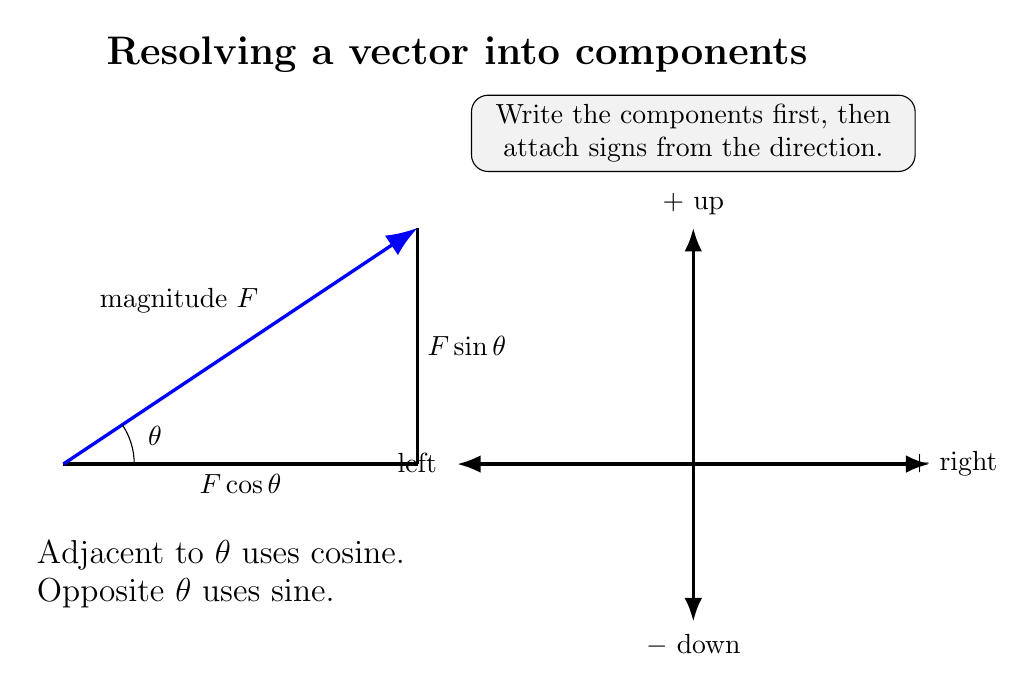
\begin{tikzpicture}[comp/.style={very thick}, vect/.style={-{Latex[length=4mm]}, very thick, blue}]
\node[font=\Large\bfseries] at (0,4.2) {Resolving a vector into components};\coordinate (A) at (-5,-1);\coordinate (B) at (-0.5,-1);\coordinate (C) at (-0.5,2);\draw[comp] (A) -- (B);\draw[comp] (B) -- (C);\draw[vect] (A) -- (C);\node[below] at (-2.75,-1) {$F\cos\theta$};\node[right] at (-0.5,0.5) {$F\sin\theta$};\node[above left] at (-2.4,0.8) {magnitude $F$};\pic [draw, "$\theta$", angle eccentricity=1.35, angle radius=0.9cm] {angle = B--A--C};\node[align=left, font=\large] at (-3,-2.4) {Adjacent to $\theta$ uses cosine.\\Opposite $\theta$ uses sine.};\draw[comp, -{Latex[length=3mm]}] (3,-1) -- (6,-1);\draw[comp, -{Latex[length=3mm]}] (3,-1) -- (0,-1);\draw[comp, -{Latex[length=3mm]}] (3,-1) -- (3,2);\draw[comp, -{Latex[length=3mm]}] (3,-1) -- (3,-3);\node at (6.3,-1) {$+$ right};\node at (-0.7,-1) {$-$ left};\node at (3,2.3) {$+$ up};\node at (3,-3.3) {$-$ down};\node[draw, rounded corners=6pt, fill=gray!10, align=center, text width=5.4cm] at (3,3.2) {Write the components first, then attach signs from the direction.};
\end{tikzpicture}
\end{document}
